\section{ParallelMesh}

%%%%%%%%%%%%%%%%%%%%%%%%%%%%%%%%%%%%%%%%%%%%%%%%%%%%%%%%%%%%%%%%%%%%%
\royslide{Mesh Classes}{

\begin{columns}
\begin{column}{.5\textwidth}
  \begin{center}
    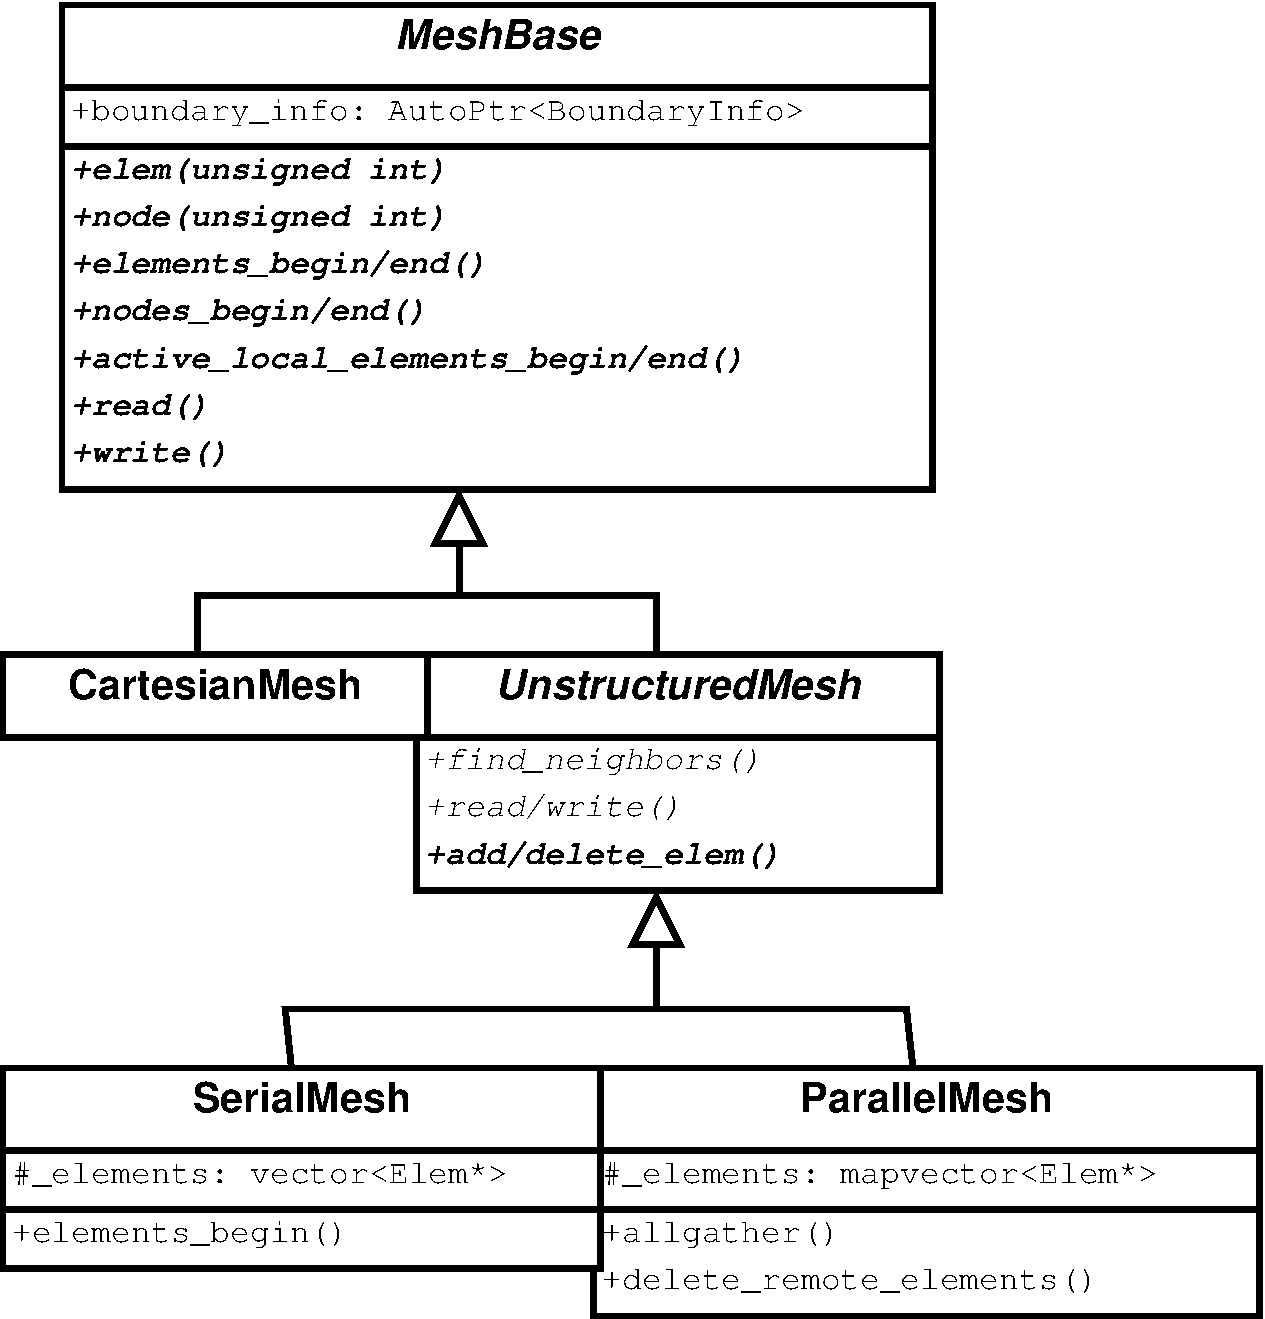
\includegraphics[width=.9\textwidth]{figs/MeshUML}
  \end{center}
\end{column}
\begin{column}{.5\textwidth}
  \royitemizebegin{}
    \item Abstract iterator interface hides mesh type from most applications
    \item UnstructuredMesh "branch" for most library code
    \item ParallelMesh implements data storage, synchronization
  \royitemizeend
\end{column}
\end{columns}
}



%%%%%%%%%%%%%%%%%%%%%%%%%%%%%%%%%%%%%%%%%%%%%%%%%%%%%%%%%%%%%%%%%%%%%
\royslide{SerialMesh Partitioning}{
\begin{columns}
\begin{column}{.5\textwidth}
  \royitemizebegin{}
    \item Each element, node is ``local'' to one processor
    \item Each processor has an identical Mesh copy
    \item Mesh stays in sync through redundant work
    \item FEM data synced on ``ghost'' elements only
  \royitemizeend
\end{column}
\begin{column}{.5\textwidth}
  \begin{center}
    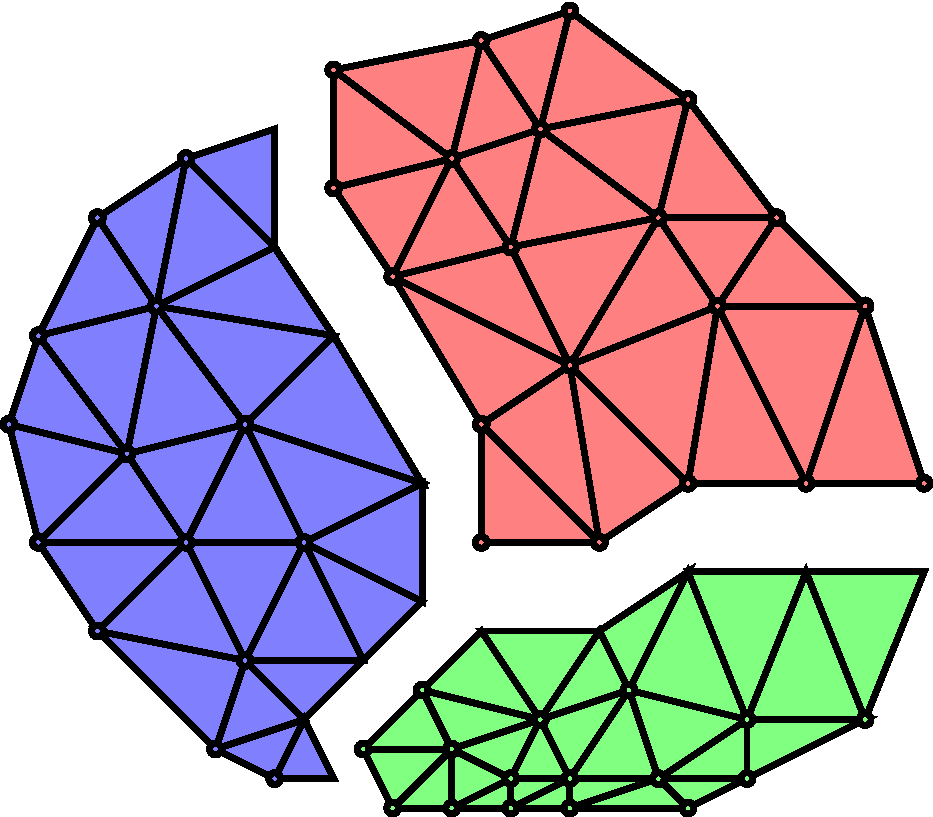
\includegraphics[width=.9\textwidth]{figs/SerialMesh}
  \end{center}
\end{column}
\end{columns}
}


%%%%%%%%%%%%%%%%%%%%%%%%%%%%%%%%%%%%%%%%%%%%%%%%%%%%%%%%%%%%%%%%%%%%%
\royslide{ParallelMesh Partitioning}{
\begin{columns}
\begin{column}{.5\textwidth}
  \royitemizebegin{}
    \item Processors store only local and ghost objects
    \item Each processor has a small Mesh subset
    \item Mesh stays in sync through MPI communication
  \royitemizeend
\end{column}
\begin{column}{.5\textwidth}
  \begin{center}
    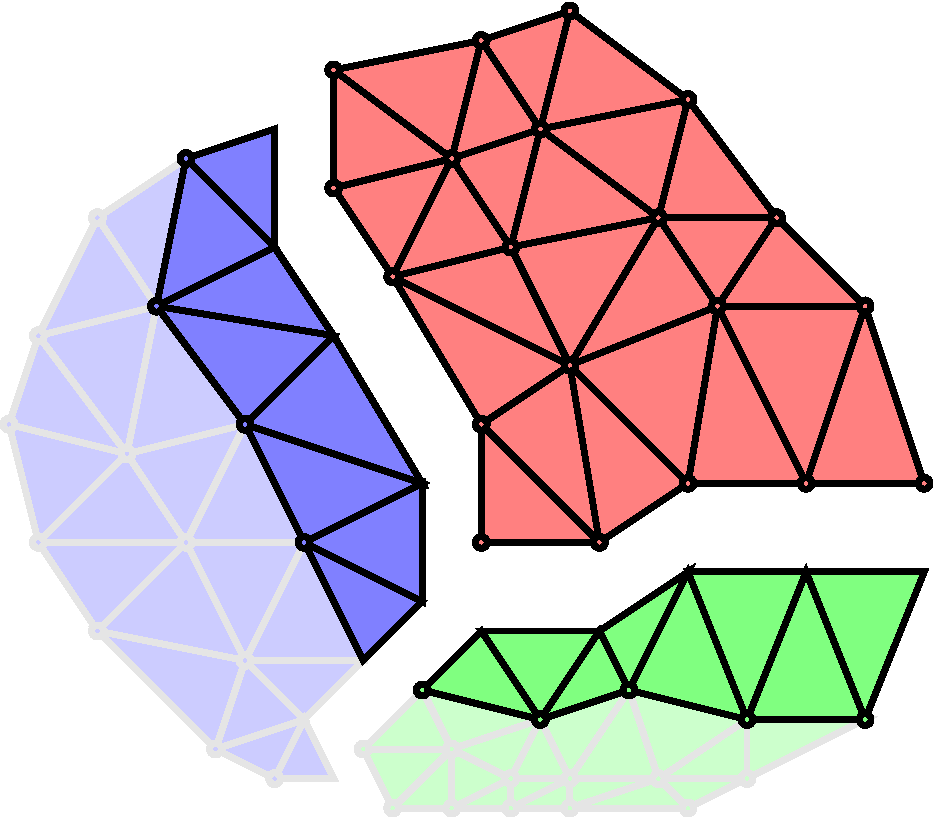
\includegraphics[width=.9\textwidth]{figs/ParallelMesh1}
  \end{center}
\end{column}
\end{columns}
}



%%%%%%%%%%%%%%%%%%%%%%%%%%%%%%%%%%%%%%%%%%%%%%%%%%%%%%%%%%%%%%%%%%%%%
\royslide{ParallelMesh Partitioning}{
\begin{columns}
\begin{column}{.5\textwidth}
  \royitemizebegin{Pros}
    \item Reduced memory use
    \item $O(N_E/N_P)$ CPU costs
  \royitemizeend
\end{column}
\begin{column}{.5\textwidth}
  \begin{center}
    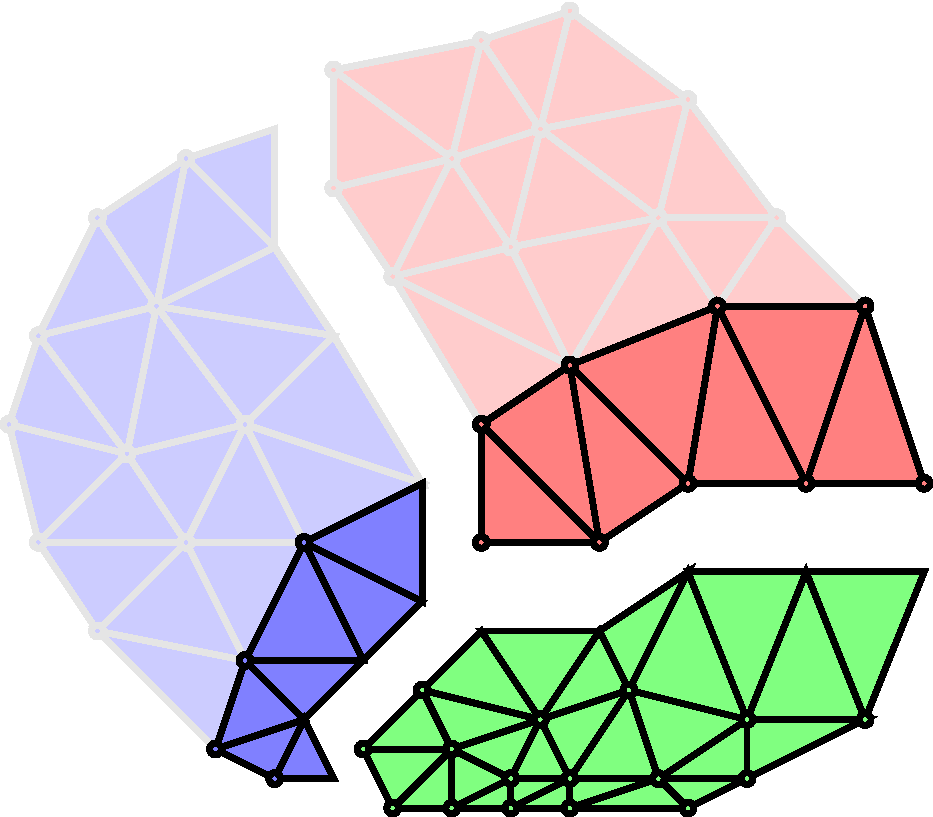
\includegraphics[width=.9\textwidth]{figs/ParallelMesh2}
  \end{center}
\end{column}
\end{columns}
}



%%%%%%%%%%%%%%%%%%%%%%%%%%%%%%%%%%%%%%%%%%%%%%%%%%%%%%%%%%%%%%%%%%%%%
\royslide{ParallelMesh Partitioning}{
\begin{columns}
\begin{column}{.5\textwidth}
  \royitemizebegin{Cons}
    \item Increased code complexity
    \item Increased synchronization ``bookkeeping''
    \item Greater debugging difficulty
  \royitemizeend
\end{column}
\begin{column}{.5\textwidth}
  \begin{center}
    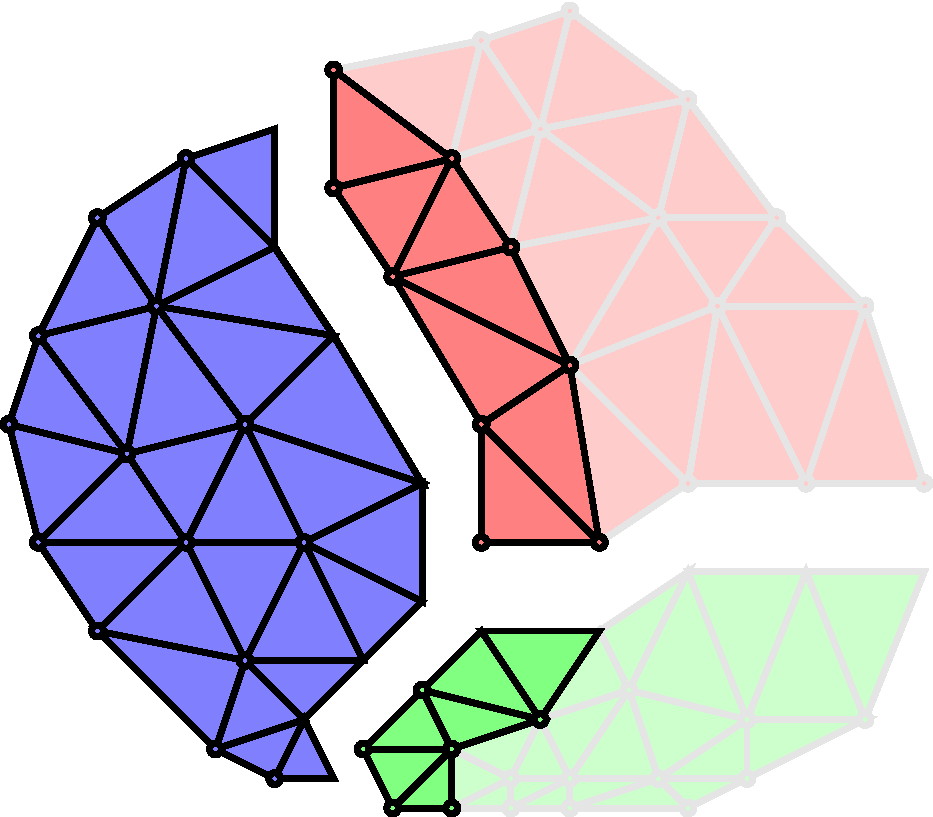
\includegraphics[width=.9\textwidth]{figs/ParallelMesh3}
  \end{center}
\end{column}
\end{columns}
}



%%%%%%%%%%%%%%%%%%%%%%%%%%%%%%%%%%%%%%%%%%%%%%%%%%%%%%%%%%%%%%%%%%%%%
\royslide{Gradual Parallelization}{
  \royitemizebegin{Starting from SerialMesh behavior}
    \item New internal data structure
    \item Methods to delete, reconstruct non-semilocal objects
    \item Parallelized DofMap methods
    \item Parallelized MeshRefinement methods
    \item Parallel Mesh I/O support
    \item Load balancing support
  \royitemizeend

  Also working on parallel support in Boundary, Function, Generation,
Modification, Generation, Tools classes
}
